\chapter{Concept}\label{Chap:Concept}

For further reading the to be built system will be called "Parametrised Augmented Reality Robot Human Interface" (\textit{PARRHI}).

\section{Goal}
As described in section \ref{Section:PARRHIApproach} this thesis presents a possible approach to solve the previously described problems (see section \ref{Section:ProblemDescription}). It is the main target of this bachelor's thesis to remove the necessity of high software engineering skills to develop reasonably complex Augmented Reality Robot Human Interface applications, maintaining the quality of the outcome and even increasing the degree of resuability. This might result in lower development costs, lower struggle to gather software engineering talent and even in a shorter time to market.

To succeed in this goal, a specific set of requirements has to be defined and documented in a formal way. To gather these requirements the V-Model developed by the Federal Republic of Germany was used~\cite{vmodell}.

\section{User Requirements}
Before defining the User Requirements the system's end user has to be defined. The characteristics of the actual enduser of \textit{PARRHI} might be someone who:
\begin{itemize}
	\setlength\itemsep{-1em}
	\item Knows the basics of text editing software,
	\item has no qualifications in software engineering,
	\item wants to develop an Augmented Reality application for professionals that collaborate with industrial robots in a shared perimeter.
\end{itemize}

Having an idea of the end-user, the user-requirements can be defined. The user wants to:
\begin{itemize}
	\setlength\itemsep{-1em}
	\item Develop a AR-applications without software engineering skills
	\item Have the tools necessary to create medium complex applications for use cases such as tutorials, maintenance instructions or other teaching purposes
	\item Build upon other people's work or projects
	\item Launch the AR-application on a suitable device
	\item Possibly use the same system on different types and brands of robots
\end{itemize}

\section{System Requirements}\label{Section:SystemRequirements}
Deriving from the previous chapter the System should:
\begin{enumerate}
	\setlength\itemsep{-1em}
	\item have input data in a non-code format.
	\item have readable and intuitive feedback on the input data.
	\item achieve reusablity by having an input in non-binary text format that allows copy and paste reproduction.
	\item support building for hand held mobile devices and head mounted Augmented Reality glasses.
	\item allow bidirectional communication (Sending commands and receiving data) with the robot's controller 
	\item allow documentation of the applications workflow
	\item be as platform independent as possible
\end{enumerate}

\clearpage
\section{PARRHI Concept}

As discussed parametrising workflows grants a multitude of benefits (see section~\ref{Section:ParametricDesignIntoduction}). Maintainability and Reusability are just some of them. By giving a system knowledge about the real world, users are relieved from some portion of the workload. In \textit{PARRHI's} case, this could mean include information about the robot's kinematics. Both, the developer of PARRHI-Applications and the end user do not have to understand robot kinematics in order to build and use costly AR applications. 

First, \textit{PARRHI} possesses a predefined model knowledge about the real world and the Fanuc Robot. The system furthermore has ways to receive information from and act on the augmented and real world. Its information input during runtime is the robot's momentary configuration and the AR-Device's position. \textit{PARRHI} uses the received information in combination with all its existing knowledge for its parametrised input data. The programmed behaviour uses its parametrised objects to generate some output, which can either be some augmented holograms presented to the user, or actual physical acts like directly commanding the robot.

Of course the instructions to the user and commands into the physical world my directly influence the AR space due to the feedback loops in the system. If something triggers a command that moves the robot, its movement can and will be tracked by the system's ability to receive external information.

How do I mean parametrised?
How is the system built (basic level)?
What is parametrised in my specific case?
How does the system interact with the real world?

\begin{figure}[h]
	\centering
	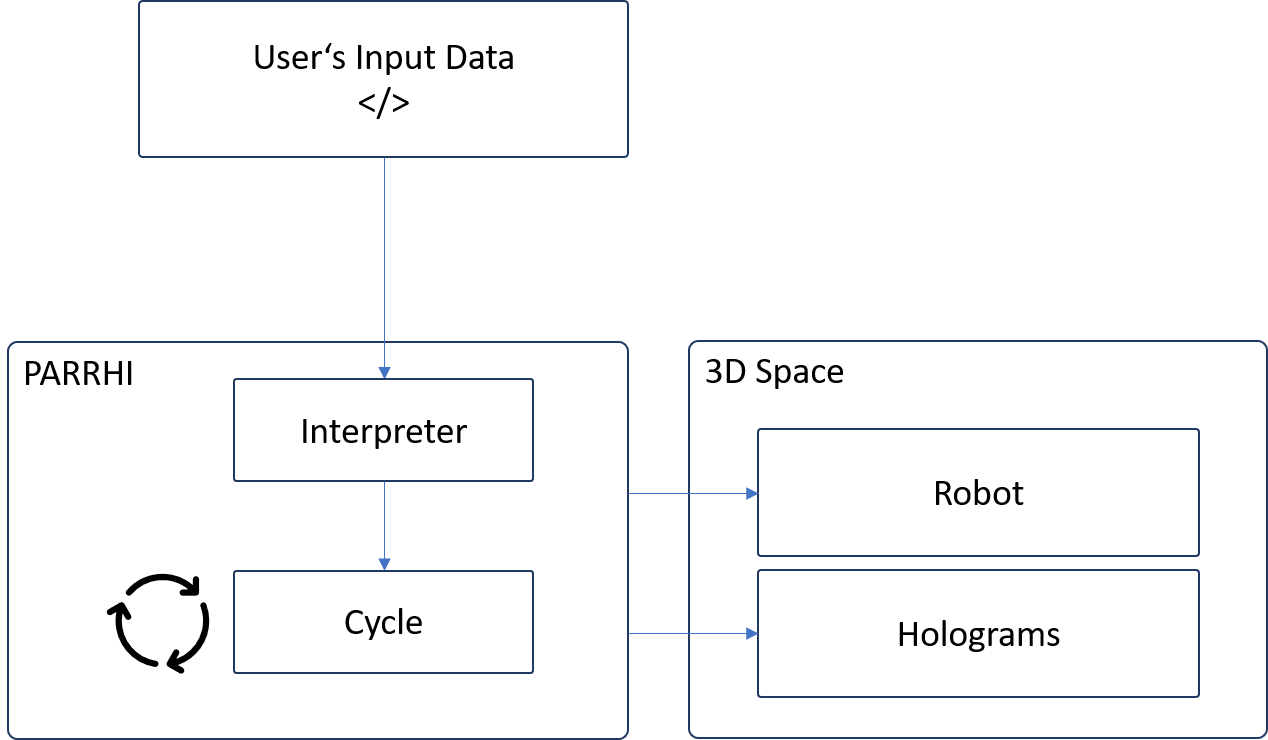
\includegraphics[width=0.75\textwidth]{Figures/PARRHIConcept01.png}
	\caption{PARRHI general concept}
	\label{Fig:PARRHIConcept}
\end{figure}

\textit{PARRHI} basically consists of three components (see Fig.~\ref{Fig:PARRHIConcept}):
\begin{enumerate}
	\setlength\itemsep{-1em}
	\item Input Data
	\item PARRHI Engine
	\item the "real world"
\end{enumerate}

\textit{Input Data} file, which is created by the application's developer, represents \textit{PARRHI's} only input. It contains a set of definitions, commands and behaviour rules that are necessary to create AR Interfaces that is able to fulfil the defined requirements in \ref{Section:SystemRequirements}.

The \textit{PARRHI Engine} interprets the input data and acts on its behalf. After validating the input data against certain schemes the engine imports all contents and sets up its internal states, before entering a cyclic mode - ready for operation.

\clearpage
\subsection{Input Data}

The Input data is the document, which the end user of the \textit{PARRHI} system constructs. It contains parametrised, hierarchically structured data, that defines the behaviour, feel and look of the final AR-HR-application. The following chapters explain the set of tools that are available to the developer, how the work and interconnect.

Table~\ref{Table:InputDataStructure} displays the top level structure and its main parts, where Variables, Points and Holograms define Utilities that Events can work with. 

\begin{table}[ht]
	\caption{\textit{Input Data} structure}
	\label{Table:InputDataStructure}
	\centering
	\begin{tabular}{lcl}
		\toprule
		Name & Section		& Explanation	\\		
		\midrule
		Variables & \ref{Section:Variables}		& Integer variables to create state machines \\
		Points& \ref{Section:Points}		& \parbox[t]{10cm}{Different kinds of 3D Point definitions\\(fix, relative to the robot, relative to the user)} 	 \\
		Holograms& \ref{Section:Holograms} & Holograms can be mounted onto points and have a set of properties\\
		Events& \ref{Section:Events} & Events have certain triggers and carry two Actions as a payload \\
		\bottomrule
	\end{tabular}
\end{table}

\subsubsection{Variables}\label{Section:Variables}
\textit{PARRHI's} variables can be used to create different steps in one's application. Variables can be the source of an event's trigger or the target of an event's action (see section~\ref{Section:Events}).

\subsubsection{Points}\label{Section:Points}
Points are a three dimensional vectors that can be defined in three different ways. 
\begin{enumerate}
	\setlength\itemsep{-1em}
	\item Fix-Point
	\item Robot-Point
	\item Camera-Point
\end{enumerate}

The \textbf{Fix-Point} has static coordinates. It could be used to setup holograms that visualize certain spacial environmental constraints or for different steps in a \textit{PARRHI} AR-HR-Interface application (see figure \ref{InputData:PointFix}).

To interact with the robot, \textit{PARRHI} needs a way to read and display data from the robot. For that, there are \textbf{Robot-Points} that are defined by two indexes of the robot's joints and one scalar value that defines the exact location between them (see figure \ref{InputData:PointRobot}). The position is calculated as follows (with s being the scalar value and J\textsubscript{n} the position vector of Joint \textit{n}):
\begin{equation}
\boldsymbol{P} = \boldsymbol{J_1} + (\boldsymbol{J_2}-\boldsymbol{J_1}) * s
\end{equation}

\textbf{Camera-Points} are a way to involve the user's position into the application. Its coordinates are periodically updated with the AR-Device's spacial position in each cycle.


\begin{figure}
	\begin{minipage}{0.45\textwidth}
		\centering
		

\tdplotsetmaincoords{60}{120} 
\begin{tikzpicture} [scale=0.01, tdplot_main_coords, axis/.style={->, black, thick}, 
vector/.style={-stealth,black,thick}, 
vector guide/.style={dashed,gray,thin}]

%standard tikz coordinate definition using x, y, z coords
\coordinate (O) at (0,0,0);

%tikz-3dplot coordinate definition using x, y, z coords

\pgfmathsetmacro{\ax}{100}
\pgfmathsetmacro{\ay}{100}
\pgfmathsetmacro{\az}{200}
\pgfmathsetmacro{\axSize}{200}

\coordinate (P) at (\ax,\ay,\az);

%draw axes
\draw[axis] (0,0,0) -- (\axSize,0,0) node[anchor=north east]{$x$};
\draw[axis] (0,0,0) -- (0,\axSize,0) node[anchor=north west]{$y$};
\draw[axis] (0,0,0) -- (0,0,\axSize) node[anchor=south]{$z$};

%draw a vector from O to P
\draw[vector] (O) -- (P);

%draw guide lines to components
\draw[vector guide]         (O) -- (\ax,\ay,0);
\draw[vector guide] (\ax,\ay,0) -- (P);
\draw[vector guide]         (P) -- (0,0,\az);
\draw[vector guide] (\ax,\ay,0) -- (0,\ay,0);
\draw[vector guide] (\ax,\ay,0) -- (0,\ay,0);
\draw[vector guide] (\ax,\ay,0) -- (\ax,0,0);
\node[tdplot_main_coords,anchor=north]
at (\ax+100,0,-60){(\ax, 0, 0)};
\node[tdplot_main_coords,anchor=west]
at (0,\ay,50){(0, \ay, 0)};
\node[tdplot_main_coords,anchor=south]
at (0,0,\az+50){(0, 0, \az)};
\end{tikzpicture}
		\caption{Fix-Point example}
		\label{InputData:PointFix}
	\end{minipage}\hfill
	\begin{minipage}{0.45\textwidth}
		\centering
		
\tdplotsetmaincoords{60}{120} 
\begin{tikzpicture}  [scale=0.03, tdplot_main_coords, axis/.style={->, black, thin}, 
vector/.style={-stealth,green,very thick}, 
robot/.style={green, very thick},
vector guide/.style={dashed,gray,thin}]

%standard tikz coordinate definition using x, y, z coords
\coordinate (O) at (0,0,0);

%tikz-3dplot coordinate definition using x, y, z coords


\pgfmathsetmacro{\axSize}{100}
\pgfmathsetmacro{\jointRadius}{50}

%Robot Points in cm (mm too large dimensions for library)
\coordinate (P0) at (0,0,0);
\coordinate (P1) at (5,0,33);
\coordinate (P2) at (5, 0, 77);
\coordinate (P3) at (15, 0, 100.5);
\coordinate (P4) at (47, 0, 100.5);
\coordinate (P5) at (55, 0, 100.5);
\coordinate (P6) at (63, 0, 100.5);
\coordinate (Point) at (5, 0 , 60);


%draw coordinate system axes
\draw[axis] (0,0,0) -- (\axSize,0,0) node[anchor=north east]{$x$};
\draw[axis] (0,0,0) -- (0,\axSize,0) node[anchor=north west]{$y$};
\draw[axis] (0,0,0) -- (0,0,\axSize) node[anchor=south]{$z$};

%draw the robot's joints and axes
\draw[robot] (P0) -- (P1); \fill[fill=gray] (P0) circle (\jointRadius pt);
\draw[robot] (P1) -- (P2); \fill[fill=gray] (P1) circle (\jointRadius pt);
\draw[robot] (P2) -- (P3); \fill[fill=gray] (P2) circle (\jointRadius pt);
\draw[robot] (P3) -- (P4); \fill[fill=gray] (P3) circle (\jointRadius pt);
\draw[robot] (P4) -- (P5); \fill[fill=gray] (P4) circle (\jointRadius pt);
\draw[robot] (P5) -- (P6); \fill[fill=gray] (P5) circle (\jointRadius pt);

%Draw PointRowot
\fill[fill=black] (Point) circle (\jointRadius pt);

%draw the 
\node[tdplot_main_coords,anchor=east]
at (P1){(Joint 1)};
\node[tdplot_main_coords,anchor=west]
at (P2){(Joint 2)};
\node[tdplot_main_coords,anchor=west]
at (Point){(Point scalar = 0.6)};




\end{tikzpicture}
		\caption{Robot-Point example}
		\label{InputData:PointRobot}
	\end{minipage}
\end{figure}


\subsubsection{Holograms}\label{Section:Holograms}
To actually augment the reality \textit{PARRHI} needs holograms. These elements have a number of attributes. Holograms can be active (respectively also inactive), have a render-mode, a geometric definition and of course a location. The locations are defined by a certain number of points - depending on the hologram's geometry. Currently the \textit{PARRHI} supports two types of holograms. There are spheres and cylinders, respectively taking one or two points and a radius as input values to define its size and position.

A Sphere's centre is always set to the point it was defined with, whereas a cylinder always connects the two points of its definition. As input points, all described types in section~\ref{Section:Points} can be used. With a given radius and point the three dimensional figure is completely defined.

Holograms have an attribute called \textit{renderMode}, which if set to "transparent", renders the hologram in a half transparent way, allowing holograms to be used for boundary or zone visualizations. Furthermore the visibility of holograms can be changed by actions as described in section~\ref{Section:Events}.

\subsubsection{Events}\label{Section:Events}
All previous elements (variables, points and holograms) exist to define the scene and to set up assets that can be utilized by events, which now actually describe the application's workflow. To do so, there are two subtypes in this category. There are event-triggers and event-actions (or short \textit{triggers} and \textit{actions}). Triggers have a boolean expression, which is checked periodically. As soon as the boolean expression evaluates to \textit{true}, the attached actions will be executed and the trigger will be disabled, avoiding multiple executions. One could say that if triggers the \textit{PARRHI's} sensors, actions are its tools to act on the augmentation. 

Triggers can be enabled and disabled, either from the beginning on, or toggled by an action. Every trigger has at least one action as a payload. To reach a reasonably capability numerous different but easy to understand triggers are available for the application's developer. In table~\ref{Table:Triggers} is a complete list of all defined triggers. \textit{(Note, that the enabled/disabled flag and actions are omitted in this table)}

 
 \begin{table}
 	\caption{Event Triggers}
 	\label{Table:Triggers}
 	\centering
 	\begin{tabular}{lll}
 		\toprule
 		Name & Input Parameter		& Trigger expression	\\		
 		\midrule
 		Distance trigger & Two Points $\boldsymbol{P_1}, \boldsymbol{P_2}$, distance $d$		&  $|\boldsymbol{P_2}-\boldsymbol{P_1}| \le d$ \\
		Variable trigger & Variable $v$, trigger value $v_{\text{tr}}$ 		& $v = v_{\text{tr}}$	 \\
		Time trigger & trigger time $t_{\text{tr}}$, time since enabling $t_{\text{enabled}}$ & $t_{\text{tr}} \geq t_{\text{enabled}}$\\
		\bottomrule
	\end{tabular}
\end{table}

\textbf{Distance trigger} can be used for two main purposes. First the application can use the robot's movement as an input using a \textit{Robot-Point}. An action could be triggered as soon as the user jogged the robot's TCP into wished position by using a \textit{Fix-Point} an waiting for them to come close to each other or to monitor the robot's configuration in Joint-Space by using two \textit{Robot-Points} as input parameters. Second the user's movement can be monitored by utilizing a \textit{Camera-Point} as an input. The application can thus ask the user to move to a specific location.

With \textbf{Variable triggers} the application is able to use defined variables as triggers. One could implement a counter for certain events, and trigger an action when a threshold value is reached. It can also be used for workflows that need states or steps. Finally the \textbf{Time trigger} allows the application to involve timers. The user could be given a maximum time for a task or holograms can be hidden after a few seconds.

Whenever a trigger's boolean expression evaluates to true, its actions are invoked and the trigger gets disabled. Since actions are the only way \textit{PARRHI} can influence the augmentation, there are numerous different types of actions - each serving a general purpose to fulfil the defined requirements (see section~\ref{Section:SystemRequirements}).

As with triggers, actions have a set of input parameters they need to fulfil their task. As with all other input data objects discussed so far, actions have a unique ID. The table~\ref{Table:Actions} gives a quick overview about all actions that \textit{PARRHI} currently supports.

\begin{table}
	\caption{Event Actions}
	\label{Table:Actions}
	\centering
	\begin{tabular}{lll}
		\toprule
		Action Name & Input Parameter		& Explanation	\\		
		\midrule
		Increment Counter  	& Variable $v$					& Increments the value of $v$ by 1 \\
		Set Hologram State 	& Hologram-IDs, State to set	& Enables/disables all specified holograms \\
		Set Trigger State  	& Trigger-IDs, State to set    	& Enables/disables all specified triggers \\
		Change UI Text	  	& Text to set					& Sets the UI Text\\
		Move Robot			& Point $P$						& Moves the robot to $P$ \\
		Set robot-hand State & State to set (open/close)		& Opens or closes the robot's gripper \\
		\bottomrule
	\end{tabular}
\end{table}

\textbf{Increment-counter actions} increment their integer variable by 1. If a developer wanted to count the number of times a user jogged the robot into a specific region, an Increment-counter action could be used as a payload of a Distance trigger. After a threshold value is reached, a Variable trigger could change the UI text and display a hint.

The \textbf{Set-Hologram-State action} enables hiding and showing holograms at runtime. If a hologram represents a region for a tutorial step, it can be hidden after the user's task is completed. The new scene can then be setup by displaying new holograms that guide the user's way. Another possible use would be, to display a warning boundary, if the user moves into a forbidden zone. This can be achieved by combining Distance trigger and Set-Hologram-State actions.

When using \textit{PARRHI} the user is presented a GUI that shows text and some other few options. The \textbf{Change-UI-Text action} allows to change this displayed text. There are numerous obvious use-cases where this is useful. Whenever it is of value to inform the user about something that cannot be achieved by holograms, this is a simple way to do so.

To create meaningful and longer applications, enabling and disabling triggers is an essential tool. This is what the \textbf{Set-Trigger-State action} is for. Triggers can only invoke their payload actions, if they are active. Triggers can either be defined as disabled from the beginning on, or get disabled by triggering as described above. The Set-Trigger-State action has the ability to (re)activate disabled triggers. There is a speciality in the case of \textit{Time triggers}. Their inner timer starts ticking, whenever they get enabled. This allows for timers to be used in the middle of applications, relative to other events.

\subsection{Interpreter}
























